\documentclass{a0poster}

\usepackage{fancytikzposter}
\usepackage{tikz}
\usepackage{xcolor}
\usepackage{titlesec}
\usepackage{array}
\usepackage[slovak]{babel}
\usepackage[utf8]{inputenc}
\usepackage[IL2]{fontenc}
\usepackage[utf8]{inputenc}
\usepackage{wrapfig}
\usepackage{xspace}
\usepackage{graphicx}




\usetemplate{2}
\usecolortemplate{2}
\useblocknodetemplate{2}
\setblockspacing{1}
\setmargin{2.5}

\usetikzlibrary{positioning, shapes, trees, graphs} % RNA trees
\usetikzlibrary{decorations.pathmorphing} % noisy shapes
\usetikzlibrary{fit}					% fitting shapes to coordinates
\usetikzlibrary{backgrounds}	% drawing the background after the foreground

\usepackage[pdftex,unicode]{hyperref}   % Musí být za všemi ostatními balíčky

\def\email{\href{mailto:richard.elias@matfyz.cz}{\nolinkurl{richard.elias@matfyz.cz}}}
\def\web{\href{http://richard.elias.matfyz.cz}{\nolinkurl{richard.elias.matfyz.cz}}}
\def\Autor{Richard Eliáš}
\def\Fakulta{Matematicko-fyzikální fakulta}
\def\Nazov{Vizualizace sekundární struktury RNA s využitím existujících struktur}

\newcommand{\Cdel}{\ensuremath{c_{del}}\xspace}
\newcommand{\Cins}{\ensuremath{c_{ins}}\xspace}
\newcommand{\Cupd}{\ensuremath{c_{upd}}\xspace}
\renewcommand{\O}[1]{\sloppy\mbox{\ensuremath{\mathcal{O}}(#1)}}
\newcommand{\scale}{0.25\textwidth}

\hypersetup{breaklinks=true}
\hypersetup{pdftitle={\Nazov}}
\hypersetup{pdfauthor={\Autor}}
\hypersetup{urlcolor=blue}


\renewcommand{\baselinestretch}{1.25} %riadkovanie
%\renewcommand{\BackgroundPicture}[0]{
  %\tikz[remember picture,overlay,opacity=.3]{
      %\node at(current page.center){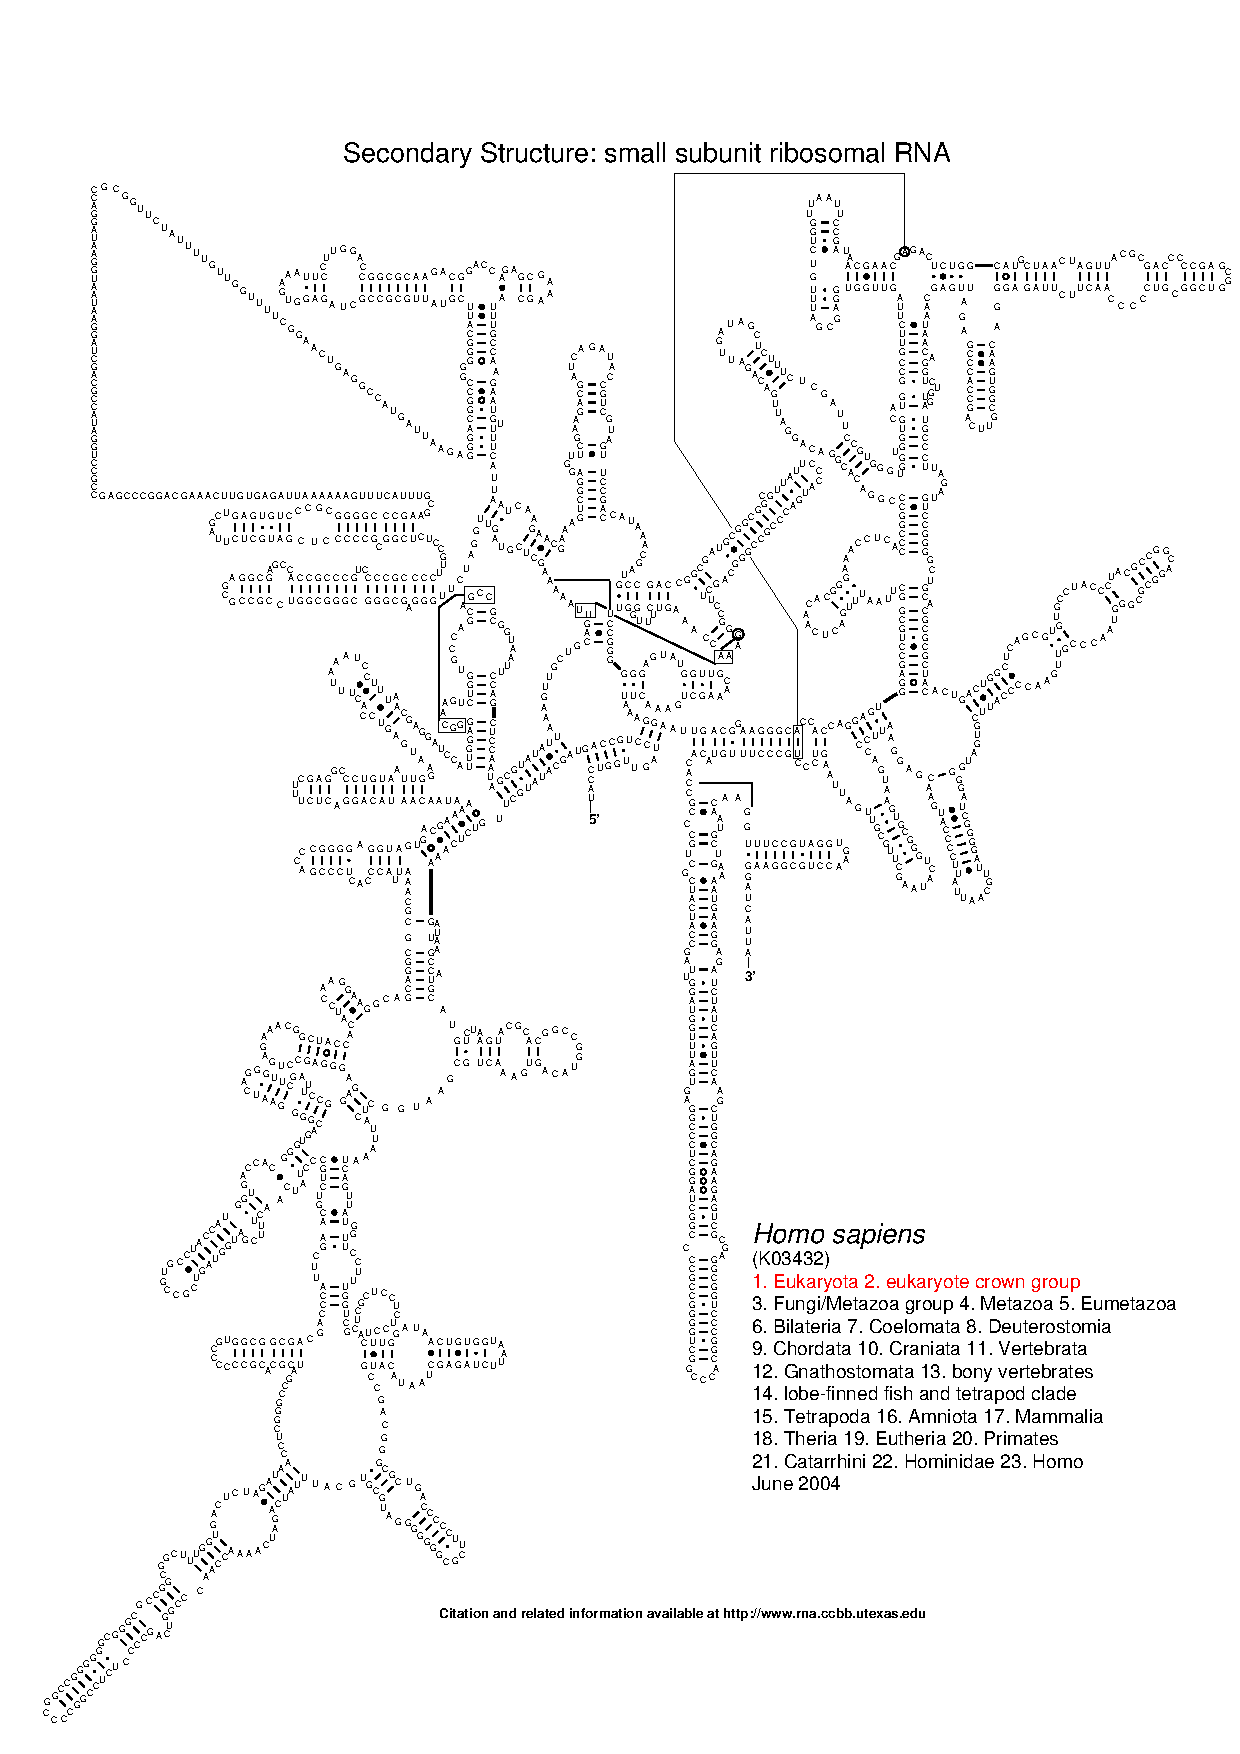
\includegraphics[height=\textheight]{../../text/img/human_crw.pdf}};
    %}
  %}



\title{\Nazov}
\author{\Autor, David Hoksza\\\Fakulta\\\texttt{\email}}
\begin{document}
\AddToShipoutPicture{\BackgroundPicture}
\noindent
\begin{tikzpicture}
  %TODO asi som nikde nespomenul co je sablona/cielova molekula
  \initializesizeandshifts
  \titleblock{50}{1}
  \blocknode{Motivácia a ciele práce}{
    Molekula RNA sa stáva predmetom mnohých štúdií, vďaka čomu rastie
    dopyt po nástrojoch pomáhajúcich pri jej analýze. Vlastnosti molekuly
    sú síce ovplyvnené primárou štruktúrou (poradím nukleotidov v~reťazci),
    no viac závisia na ich priestorovom usporiadaní (terciárna štruktára).
    My sa v~práci zaoberáme trochu zjednodušeným modelom - sekundárnou
    štruktúrou. Tú reprezentuje zoznam nukleotidov spojených väzbou.
    Tieto nukleotidy musia byť blízko aj v~priestore a~tak nám sekundárna štruktúra
    relatívne dobre aproximuje terciárnu, pre ktorú neexistujú spoľahlivé
    metódy zisťovania štruktúry už ani pre relatívne malé molekuly.

    Prvým krokom pri analýze RNA molekuly je často rozbor obrázka jej sekundárnej
    štruktúry. Medzi základné kritéria ktoré musia obrázky molekúl spľňať
    patrí rovinnosť nakreslenia, kreslenie loopov na kružnice a~stemy na priamkách.
    Pri porovnávaní štruktúr sa využíva taktiež kreslenie častí majúcich podobnú
    funkciu a~tvar na rovnaké miesta v~obrázkoch, čo pomáha lepšej orientácií
    v~molekule a~napomáha nájsť konzervované časti v~molekulách.
    V súčastných nástrojoch (mFold, RNAViz, RNAView, $\cdots$) sa toto posledné
    kritérium nedodržuje, čo má za následok ťažké nachádzanie konzervovaných častí
    v molekulách.
  }

  \renewcommand{\scale}{0.25\textwidth}
  \blocknode{Kreslenie chýbajúcich častí v molekule}{
    Po transformácií šablónovej molekuly na cieľovú, získavame čiastočnú vizualizáciu
    cieľovej RNA a jej zvyšok potrebujeme dopočítať. Po operáciách delete nám v obrázku
    ostávajú prázdne miesta, naopak po insertoch potrebujeme pre dané vrcholy urobiť
    v obrázku miesto.

    \begin{wrapfigure}{L}{0.27\textwidth}
      \begin{tikzpicture}[
          every node/.style = {rectangle, fill = none, draw = none}]
          \node (tree) {
            %trim=left bottom right top
            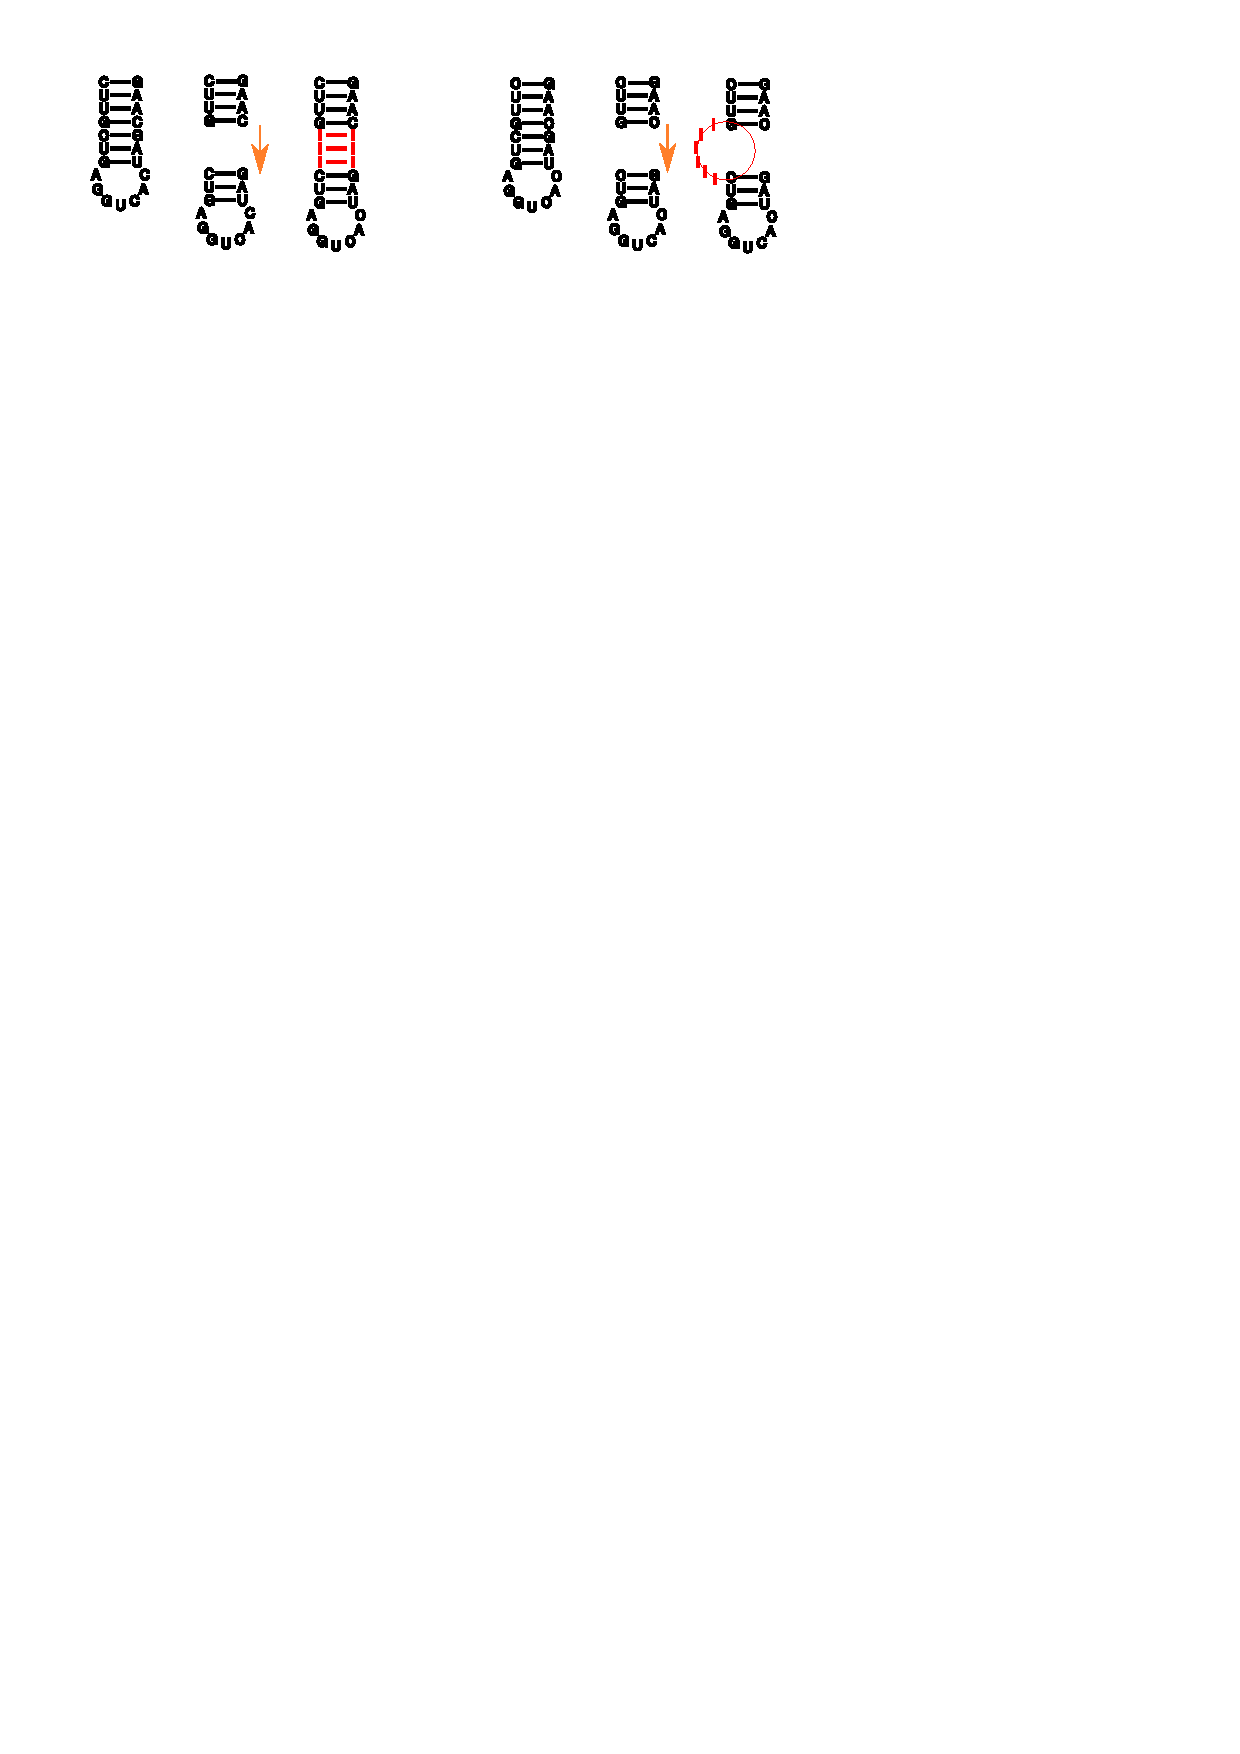
\includegraphics[clip, trim = 1cm 25cm 7cm 1cm, width=\scale]{./include/stem}
          };
      \end{tikzpicture}
    \end{wrapfigure}

    Mazanie vrcholov stromu je inverzná operácia ku vkladaniu a tak si ukážeme iba vkladnie.
    Vkladanie báz do loopu (okrem multibranch) je jednoduché, vytvoríme si iba novú kružnicu na ktorú všetky
    bázy uložíme. Vkladanie báz do stemu potrebuje najprv urobiť pre nich najprv urobiť
    miesto a tak celú štruktúru posunie smerom od rodičovského vrcholu stromu.
    Algoritmus vkladania je uvedený na obrázku.

    Pre multibranch loopy je to trochu zložitejšie, chceme sa totiž vyhnúť prípadom, kedy ju musíme
    celú prekresliť, keďže pri tom vznikajú veľké problémy s prekryvmi.
    Prekresleniu štruktúry sa nevyhneme, ak sa jedná o vkladanie veľkého počtu báz, alebo
    vkladáme celú novú vetvu RNA.
  }

  \renewcommand{\scale}{0.35\textwidth}
  \blocknode{Príklady výslednej vizualizácie (človek (K03432) a žaba (X04025), mušľa (L24489) a cikáda (U06478))}{
    \begin{tikzpicture}[
        on grid,
        node distance = 27cm,
        every node/.style = {rectangle, fill = none, draw = none}]
        \node (tree) {
          %trim=left bottom right top
          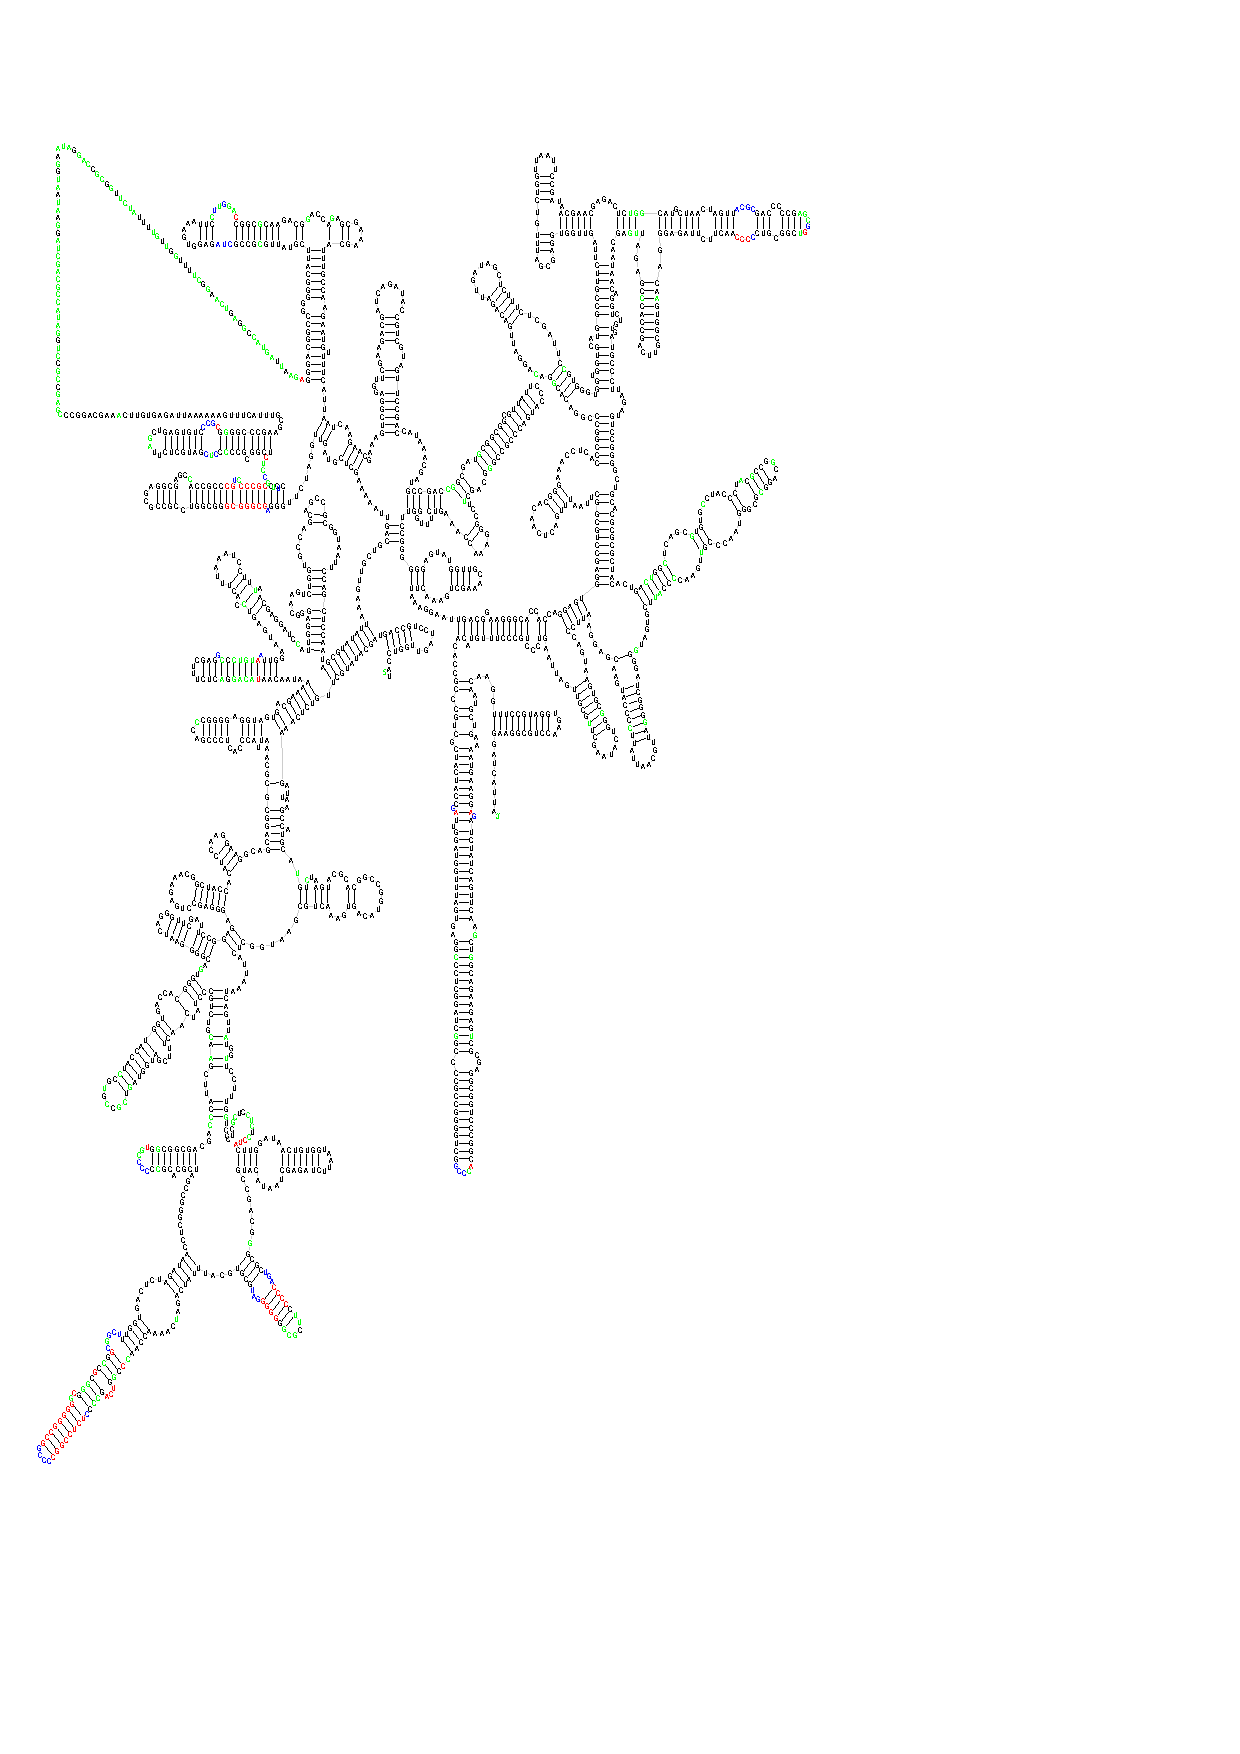
\includegraphics[clip, trim = 0 4cm 7cm 2cm, width=\scale]{./include/human-DRAW-TO-african_frog}
        };
        \node [right = of tree]{
          %trim=left bottom right top
          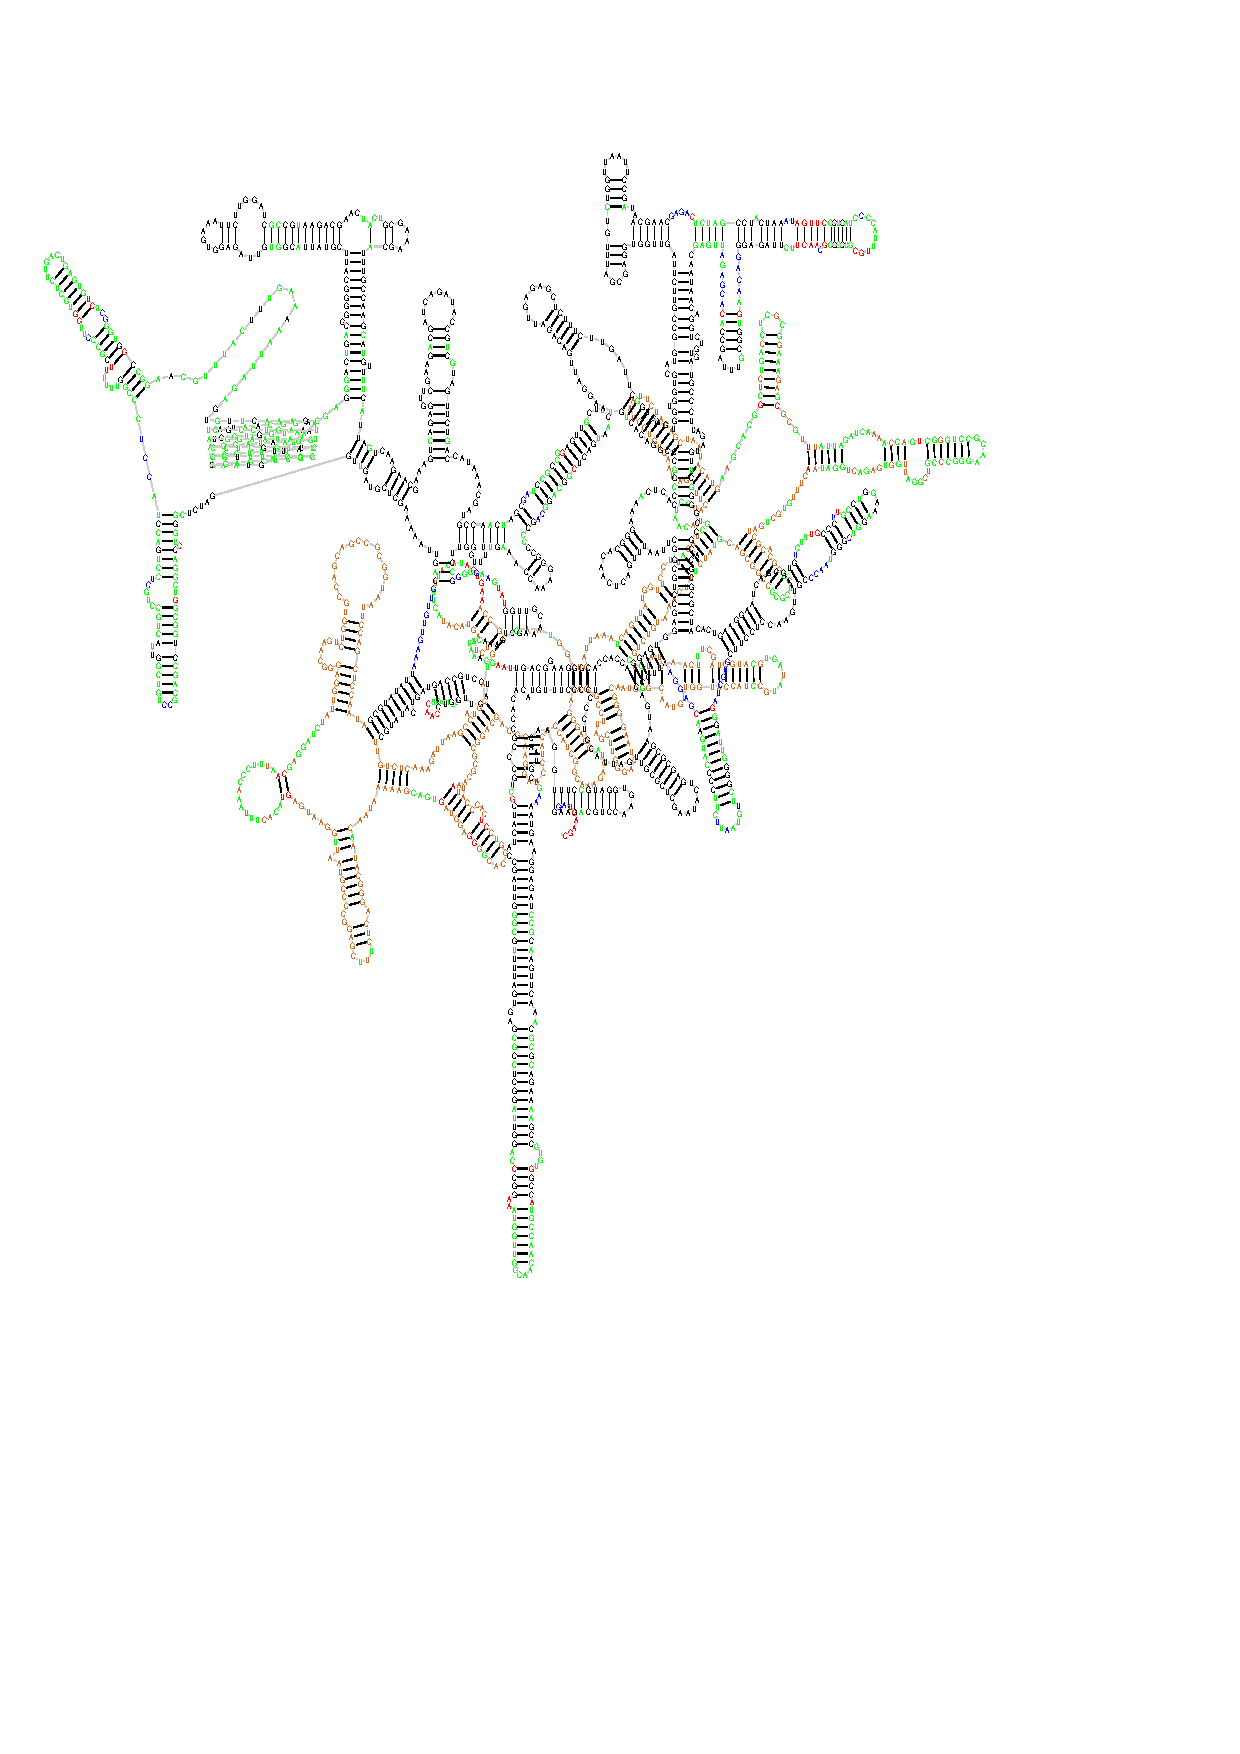
\includegraphics[clip, trim = 0 4cm 7cm 2cm, width=\scale]{./include/blue_mussel-DRAW-TO-cicadas}
        };
    \end{tikzpicture}
  }

  %\renewcommand{\scale}{6cm}
  %\blocknodew[($(-12, 0)$)]{24}{}{
    %\vspace{-3cm}
    %\begin{tikzpicture}[
        %on grid,
        %node distance = 9cm,
        %every node/.style = {rectangle, fill = none, draw = none}]
        %\node (first) {
          %%trim=left bottom right top
          %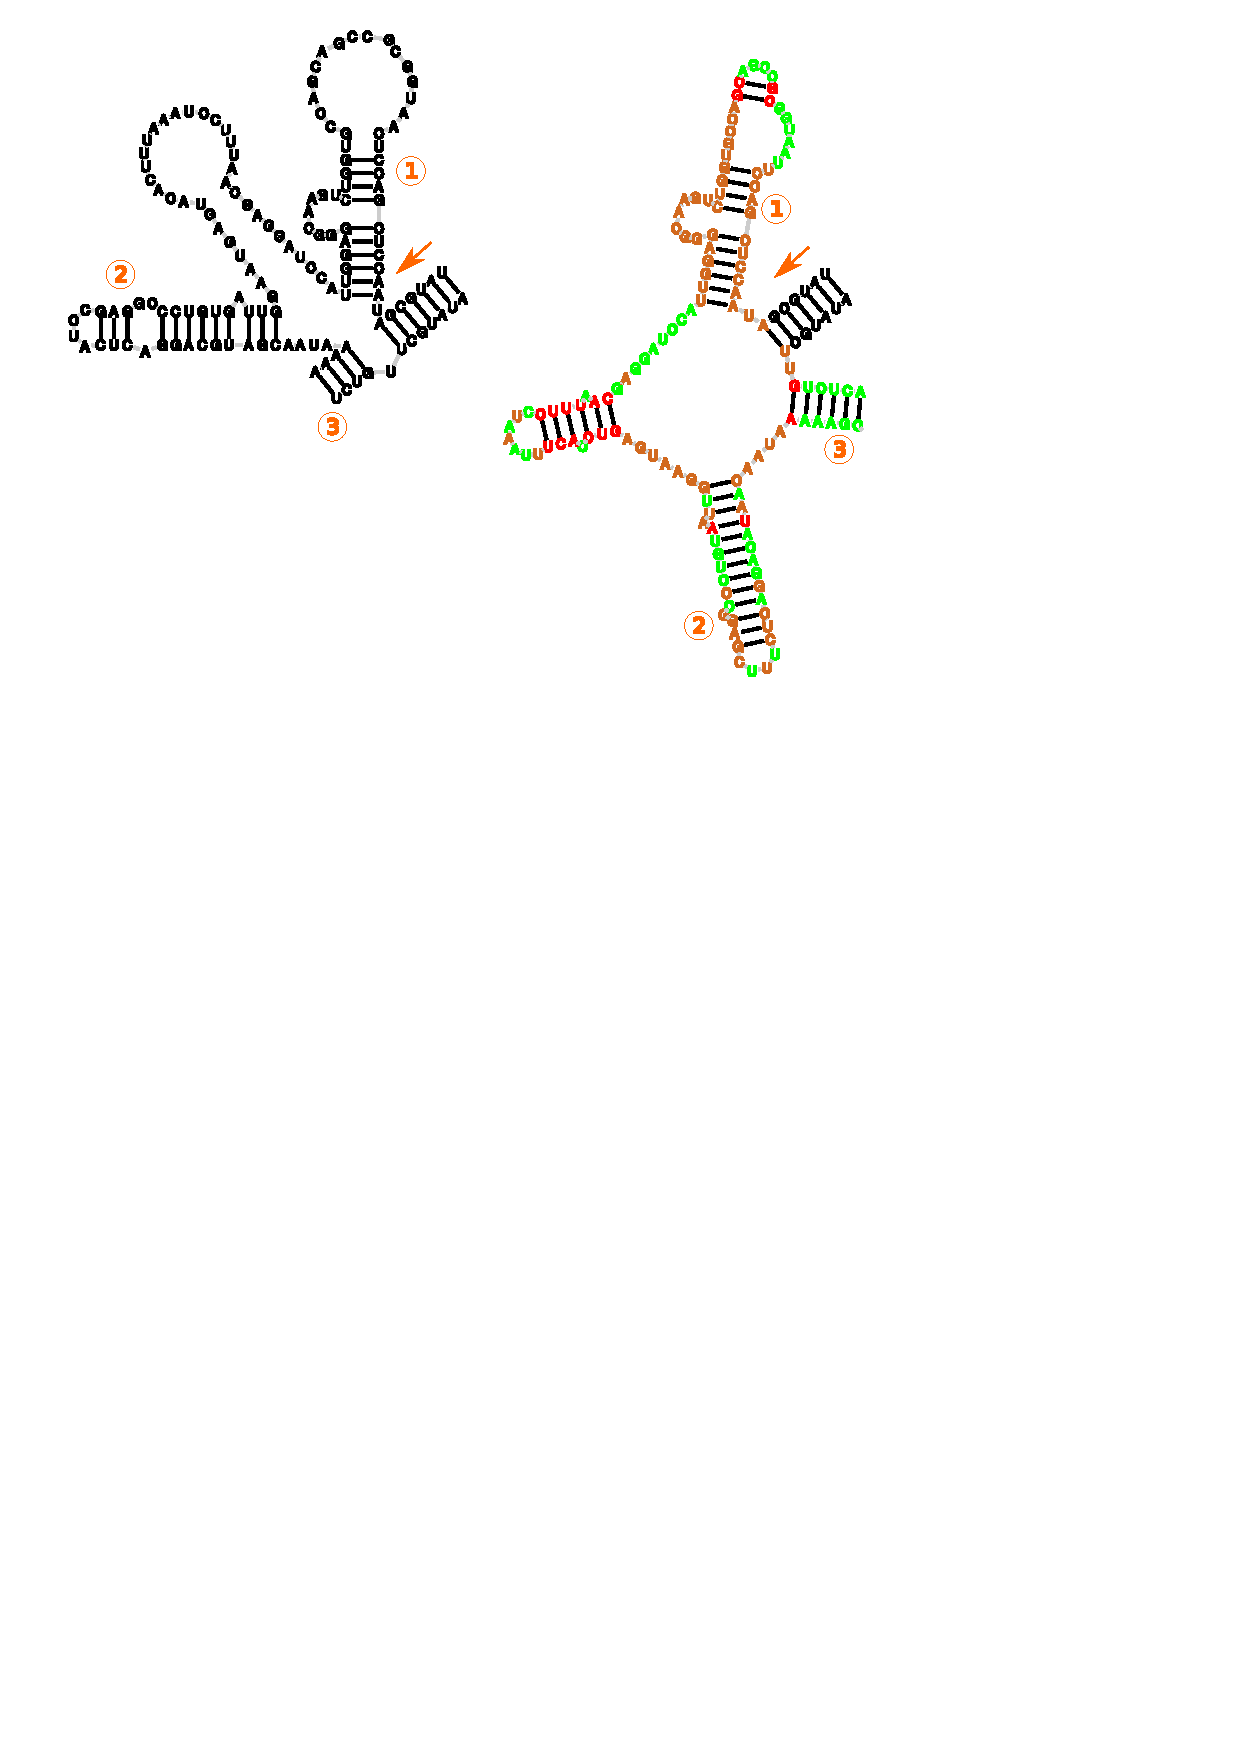
\includegraphics[clip, trim=8cm 18cm 5cm 0, width=\scale]{./include/multibranch-redraw}
        %};
        %\node [right = of first] {
          %%trim=left bottom right top
          %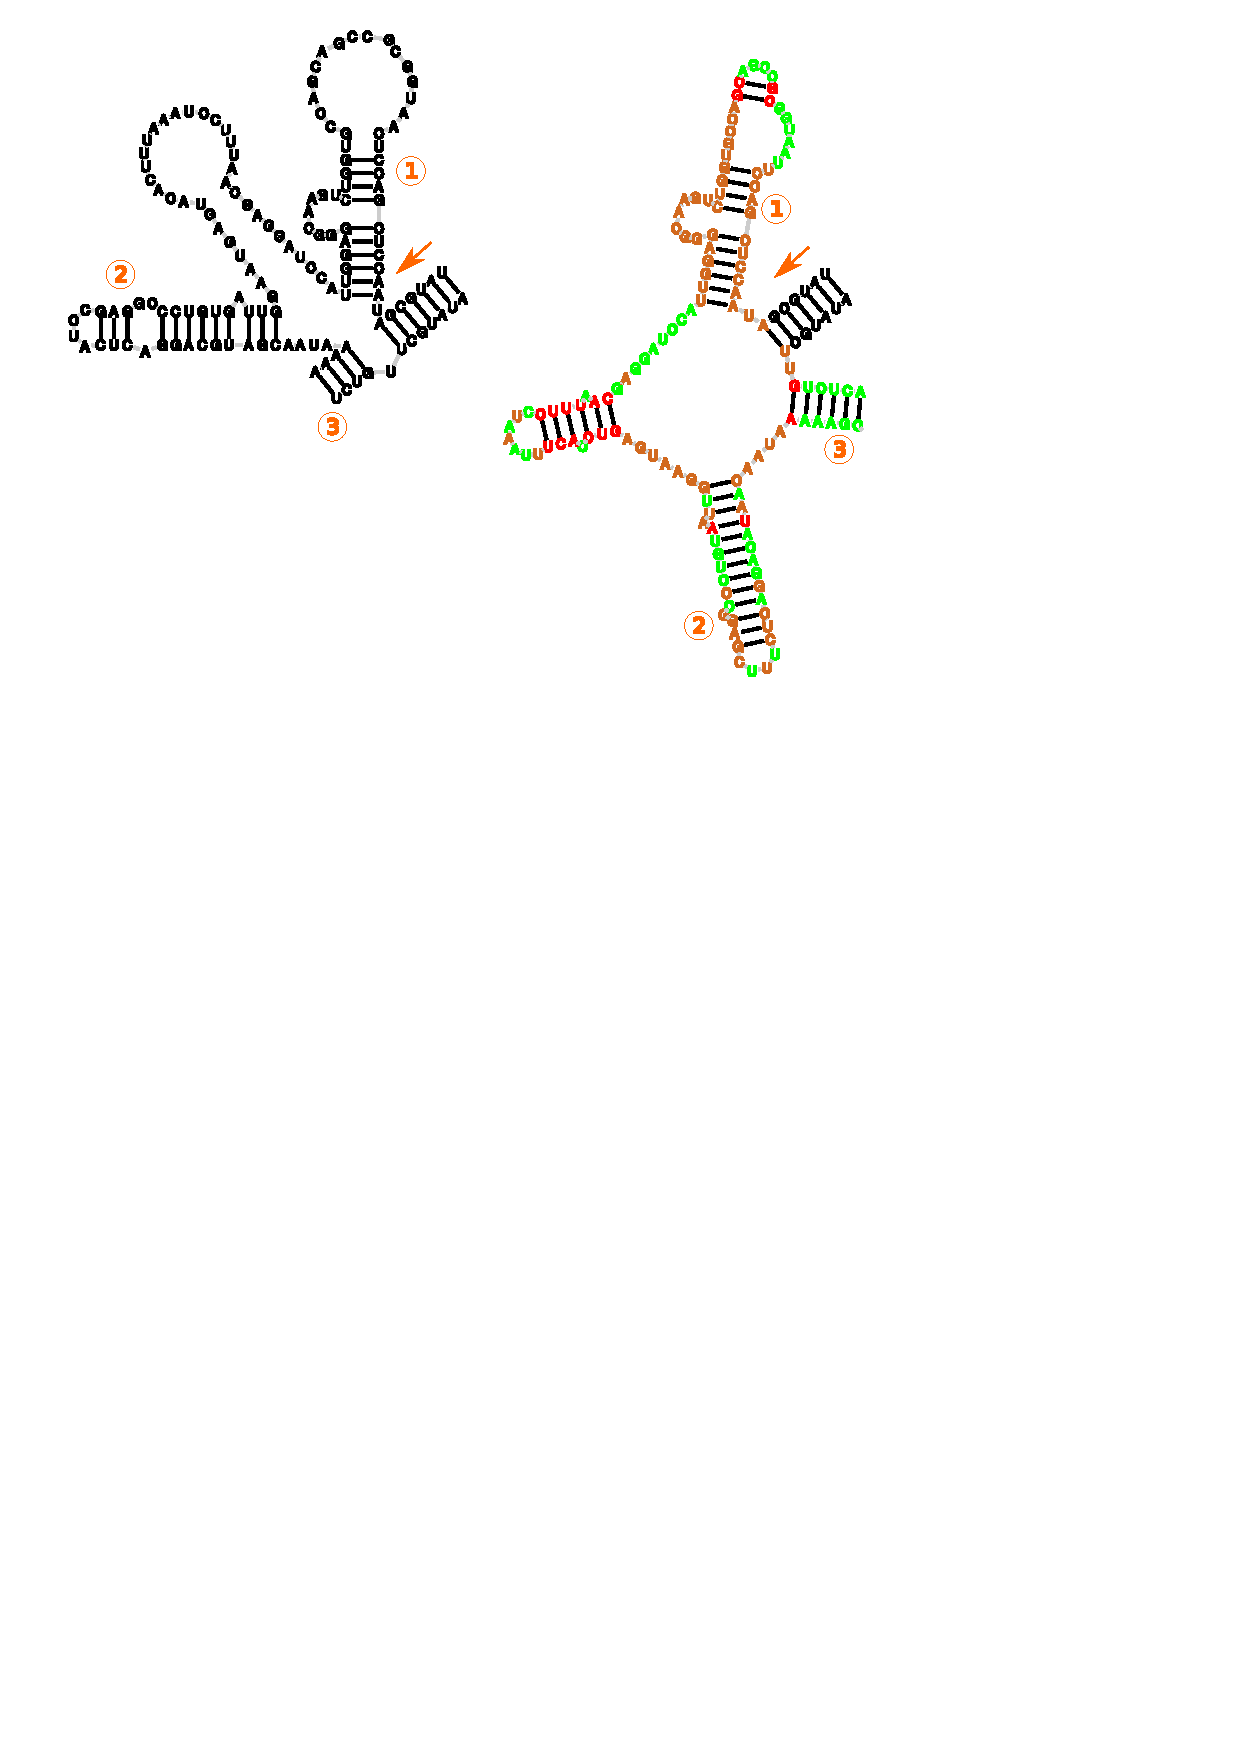
\includegraphics[clip, trim=1cm 18cm 13cm 0, width=\scale]{./include/multibranch-redraw}
        %};
    %\end{tikzpicture}
  %}


  \startsecondcolumn

  \renewcommand{\scale}{0.25\textwidth}
  \blocknode{Stromová reprezentácia RNA a použitie tree-edit-distance algoritmu}{
    \begin{wrapfigure}{L}{0.28\textwidth}
      \begin{tikzpicture}[
          on grid,
          node distance = 9cm,
          every node/.style = {rectangle, fill = none, draw = none}]
          \node (tree) {
            %trim=left bottom right top
            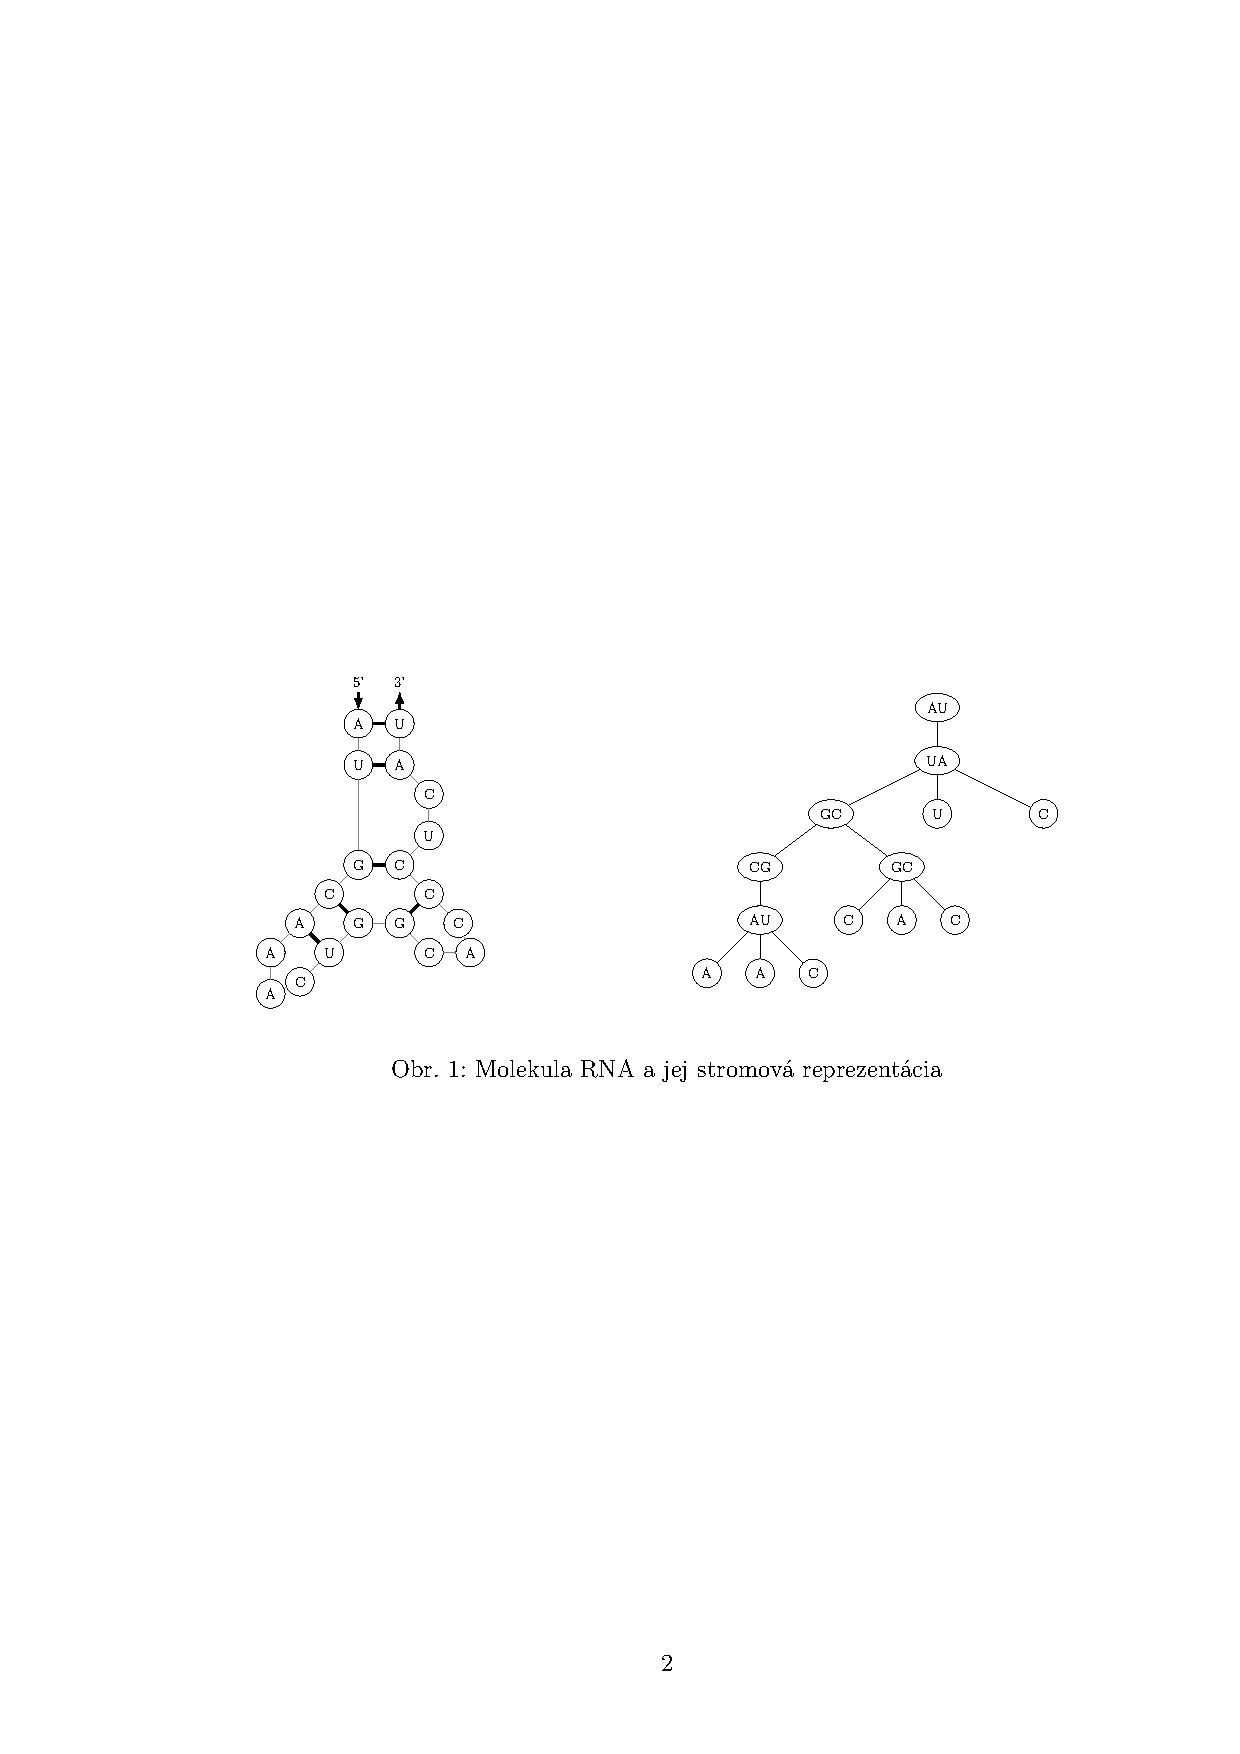
\includegraphics[clip, trim = 4cm 12cm 3cm 11cm, width=\scale]{./include/rna_tree}
          };
          \node [below = of tree]{
            %trim=left bottom right top
            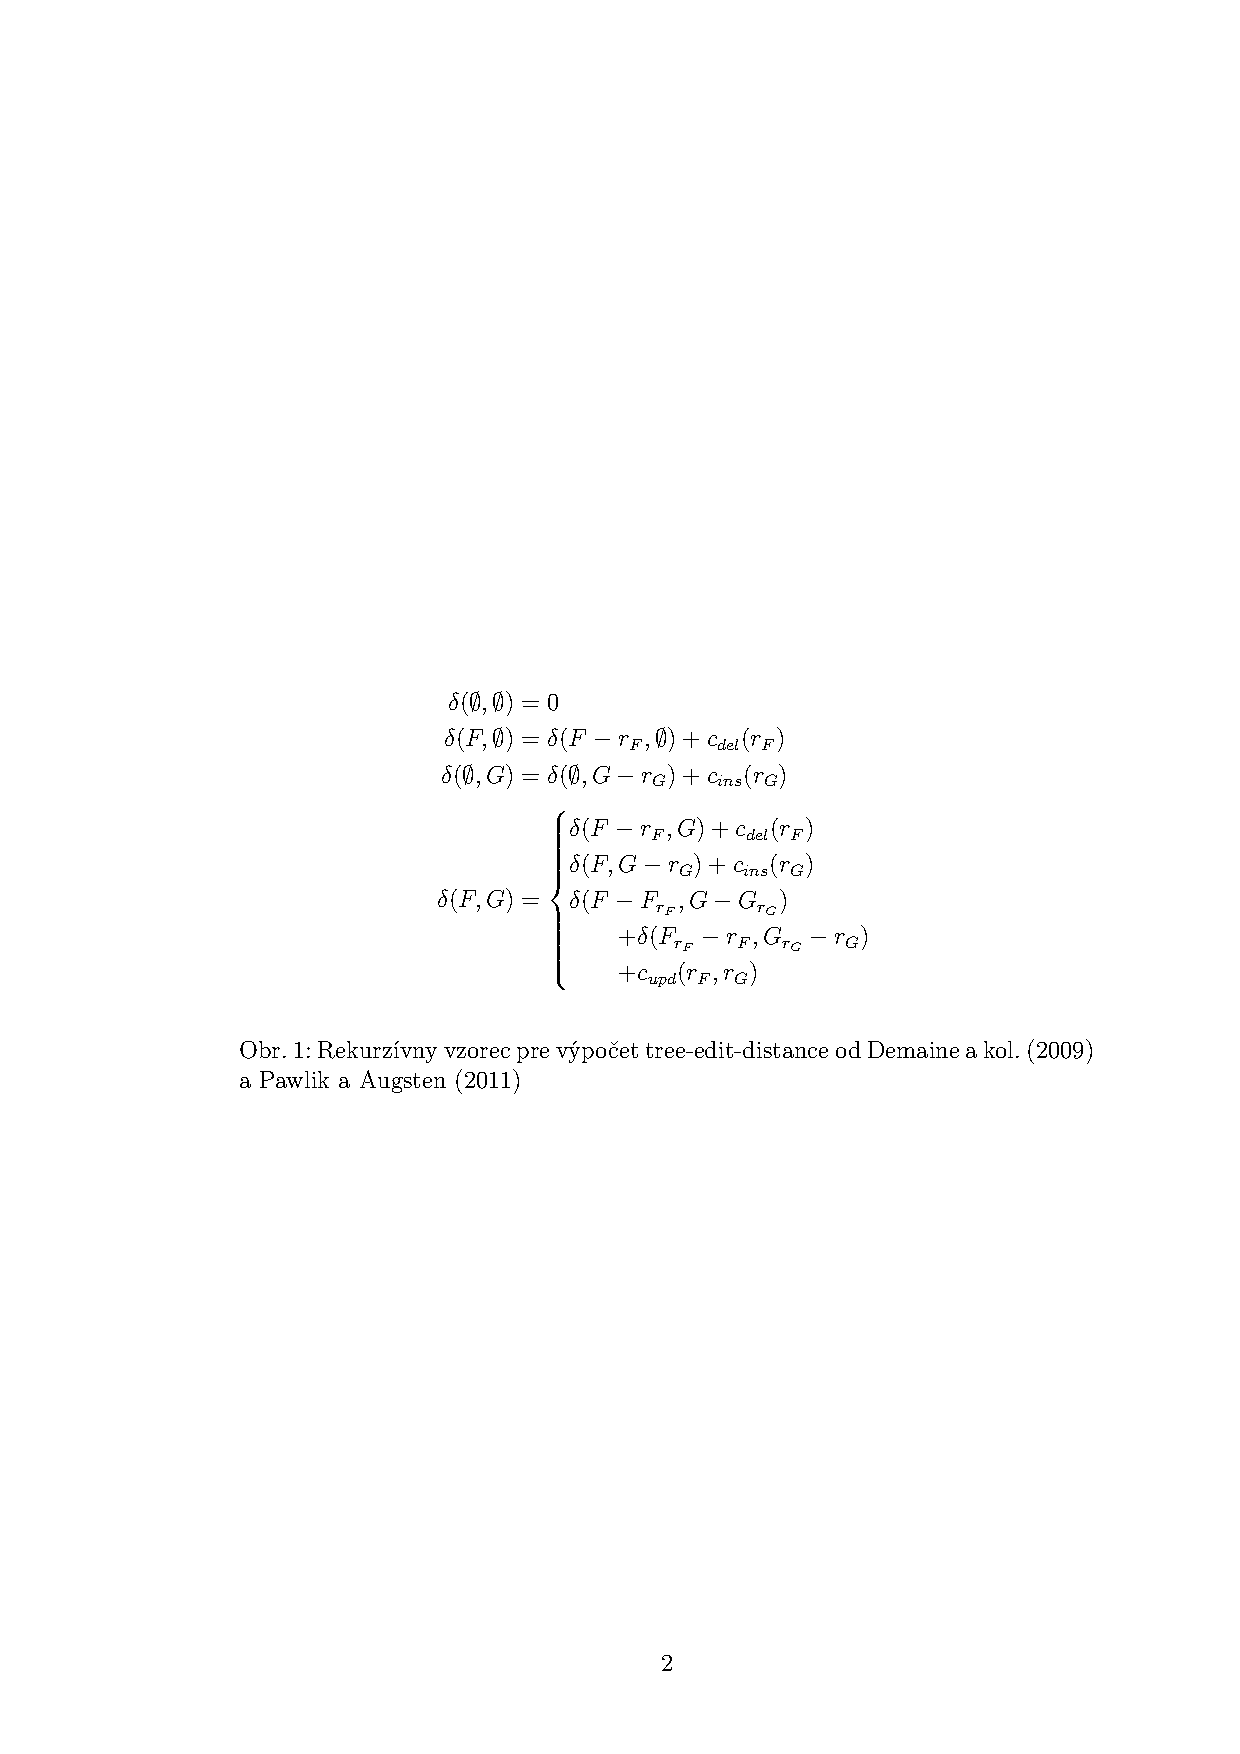
\includegraphics[clip, trim = 7cm 12.5cm 6cm 11cm, width=\scale]{./include/ted}
          };
      \end{tikzpicture}
    \end{wrapfigure}

    Vďaka zanedbaniu existencie pseudouzlov, môžeme sekundárnu štruktúru reprezentovať
    ako usporiadaný zakorenený strom (pseudouzly sú páry vedúce medzi vetvami stromu).
    Transformácia sekundárnej štruktúry do stromovej podoby je na obrázku.
    Vnútorný vrchol stromu reprezentuje bázový pár a listy nespárované nukleotidy.

    Pôvodným nakreslením chceme hýbať čo najmenej a tak potrebujeme spôsob ako
    odlíšiť časti, ktoré sa v oboch molekulách nemenia. K tomu využijeme algoritmus
    \textit{tree-edit-distance}, ktorý nám dá návod ako určiť najmenší počet úprav,
    ktorými vieme transformovať šablónovú molekulu na cieľovú.
    Úpravami myslíme editačné operácie update, insert a delete (zmena bázy vo vrchole,
    vloženie lebo zmazanie vrcholu).

    Základom algoritmu je rekurzívny vzorec, ktorý určí vzdialenosť medzi dvoma lesmi
    ($r_{F}$ a $r_{G}$ označuje najpravejší, alebo najľavejší vrchol lesa $F$ a $G$,
    \Cdel, \Cins, \Cupd sú ceny mazania, vkladania a updatu vrcholu v strome).
    Využitím algoritmu \textit{RTED} môžeme vzdialenosť medzi stromami spočítať
    v čase \O{$n^3$}. Ten nám totiž vie predpočítať optimálnu dekompozíciu,
    teda do ktorej vetvy rekurzie sa zanoriť, a ktorú naopak vynechať.

    Bolo dokázané, že pre každú dekompozičnú stratégiu existujú stromy, ktoré
    potrebujú aspoň \O{$n^3$} času a tak je tento algoritmus optimálny.

    Nakoniec, algoritmus \textit{TED} nám dáva návod ako stromy navzájom transformovať
    jeden na druhý. Ide len o pamätanie si, že ak som v nejakom kroku rekurzie vrchol
    mazal, tak ho potrebujem zmazať aj pri transformácií. Obdobne je to aj s ostatnými
    operáciami.
  }
  \blocknode{Nástroj TRAVeLer}{
    V rámci práce sme implementovali nástroj TRAVeLer, ktorý je schopný podľa vstupného
    obrázka vizualizovať cieľovú štruktúru.

    Program implementuje \textit{tree-edit-distance} algoritmus, ktorý nám zabezpečí
    správne mapovanie medzi vzorovou a cieľovou štruktúrou.
    Následným použitím nášho dokresľovacieho algoritmu vznikne výsledná vizualizácia.

    V nasledujúcich príkladoch uvažujeme premenné
    \mbox{INDIR=../InFiles/} a \mbox{OUTDIR=/tmp/}.

    Príklad 1: generovanie vizualizácie RNA myši pomocou obrázka RNA človeka

    \coloredbox{colorthree!50!}{
      \# ./build/traveler
           --match-tree \$INDIR/mouse.fasta
           --template-tree \$INDIR/human.ps \$INDIR/human.fasta
           --all \$OUTDIR/mouse\_to\_human
    }

    Príklad 2: získavanie mapovania medzi štruktúrami

    \coloredbox{colorthree!50!}{
      \# ./build/traveler
           --match-tree \$INDIR/mouse.fasta
           --template-tree \$INDIR/human.ps \$INDIR/human.fasta \textbackslash \\ \mbox{\hspace{1.5cm}}
           --ted \$OUTDIR/mouse\_to\_human.map
    }

    Príklad 3: generovanie vizualizácie z existujúceho mapovania

    \coloredbox{colorthree!50!}{
      \# ./build/traveler
           --match-tree \$INDIR/mouse.fasta
           --template-tree \$INDIR/human.ps \$INDIR/human.fasta \textbackslash \\ \mbox{\hspace{1.5cm}}
           --draw --colored --overlaps \$INDIR/mouse\_to\_human.map \$OUTDIR/mouse\_to\_human
    }

    Argumentom \textit{--colored} zapíname farebné kódovanie v obrázku: \textbf{červená} - insert,
    \textbf{zelená} - edit, \textbf{modrá} - prekreslenie báz, \textbf{hnedá} - prekreslenie multibranch loopy.
  }
  \blocknode{Výsledky experimentov}{
    Program sme testovali na reálnych dátach z CRW databázy. Ako testovaciu sadu sme zvolili malú podjednotku
    16S ribozomálnej RNA v živočíšnej ríši. V databáze je ulozených 16 molekúl (kompletných - obrázok aj štruktúra),
    z ktorých sme získali 256 výsledných vizualizácií (každý s každým).

    V počte prekryvov sme sa u väčšiny prípadov držali počtu do 10 (151), ak vynecháme molekuly ktoré potrebovali
    prekresliť multibranch loopy, tak do 10 prekryvov bolo nakreslených 150 molekúl a nad 10 ich bolo iba 29.

    Počty prekryvov v závislosti na vzdialenosti TED nieje štatisticky až taká zjavná. Ak vezmeme najbližšie
    štruktúry, je v priemere asi 5 prekryvov a so zväčšujúcou sa vzdialenosťou rástli výkyvy hlavne kvôli tomu,
    že niektoré štruktúry boli dobre konzervované a na druhej strane bolo pár extrémov, ktoré sa vizualizovali
    veľmi ťažko.

    V budúcnosti by bolo vhodné upraviť kresliace algoritmy, implementovať otáčanie vetiev RNA stromov v prípade
    indikovania prekryvov alebo pridať interaktívny nástroj na úpravu obrázkov, čím by užívateľ prekryvy ručne
    odstránil.
  }
\end{tikzpicture}
\end{document}
